\chapter{LabVIEW and Arduino}
If you have covered Chapter 2 \& 3, you are more than ready to start using $\labview$ to manipulate real world objects. Although this chapter would be largely self contained, it is assumed that you have covered chapter 1 and understand the basics of $\labview$. Where relevant, you will be referred to chapter 2 or the $\labview$ helpfiles in order to aid you through examples\\

This chapter will focus on the ``LiNX'' package, it should be installed with your community edition of $\labview$. To check if you do have this package installed, go to the block diagram and open the functions palette. Near the bottom of the menu, you will see a folder called ``Hobbyist", this contains all the functions you need to talk to your Arduino board. If it is not installed, you can use the JKI package manager to install it.
\section{Getting Started}
Before we begin sending commands to our Arduino board, we need to flash specific firmware onto the little microcontroller of the board. To do this, you need the LiNX firmware wizard. You can open the firmware wizard by going to ``Tools'' on the taskbar and selecting Firmware from the menu.\\ %TODO, CHECK THIS

Before you move along, the rest of the chapter assumes you will be using an Arduino Uno, I have tested it on an Arduino Nano before so your mileage may vary. Since the firmware wizard does not have much in the way of troubleshooting options, you should make sure that you can flash programs onto your device using the Arduino Studio program. Make note of the serial address, you will need it for the next step.\\

Figure \ref{FirmwareTool} shows the wizard open, use the following settings: (Assuming you will be using an Arduino Uno)
\begin{itemize}
	\item \textbf{Device Family}: Arduino
	\item \textbf{Device Type}: Arduino Uno
	\item \textbf{Firmware Update Method}: Serial / USB
\end{itemize}
\begin{figure}
	\centering
	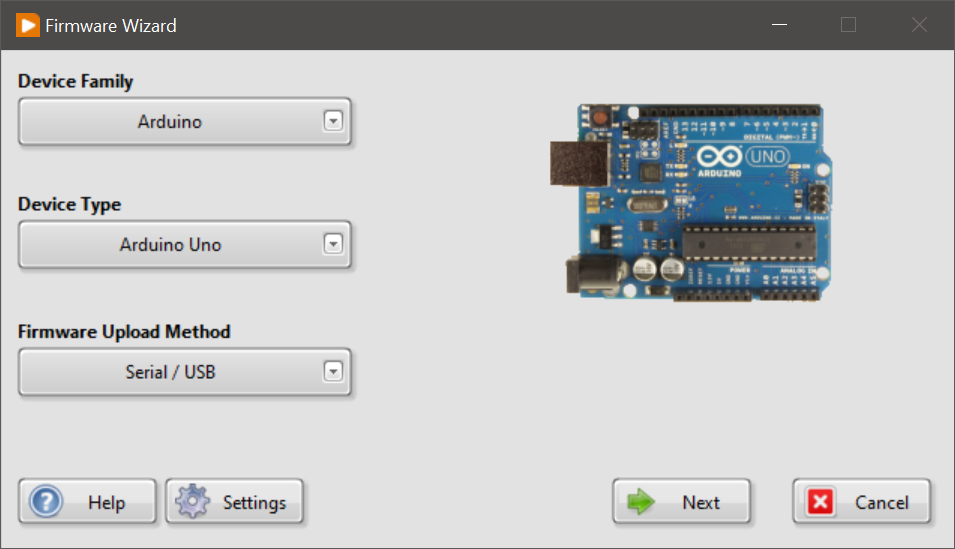
\includegraphics[width=0.75\textwidth]{FirmwareTool}
	\caption{The LiNX firmware wizard, we use this tool to make the Arduino learn $\labview$.}
	\label{FirmwareTool}
\end{figure}
In the settings menu, make sure that you have the correct port selected which is connected to your device %TODO, go over this part
\section{Writing and Reading Ports}

\section{Quite Advanced Projects}